\chapter{Multi-armed Bandits}\label{ch-multi-armed}


\begin{figure}[h!]
\centering
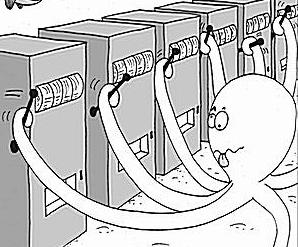
\includegraphics[width=3in]
{multi-armed/octupus-bandit.png}
\caption{Multi-armed bandit (MAB).
} 
\label{fig-octupus-bandit}
\end{figure}

\begin{figure}[h!]
\centering
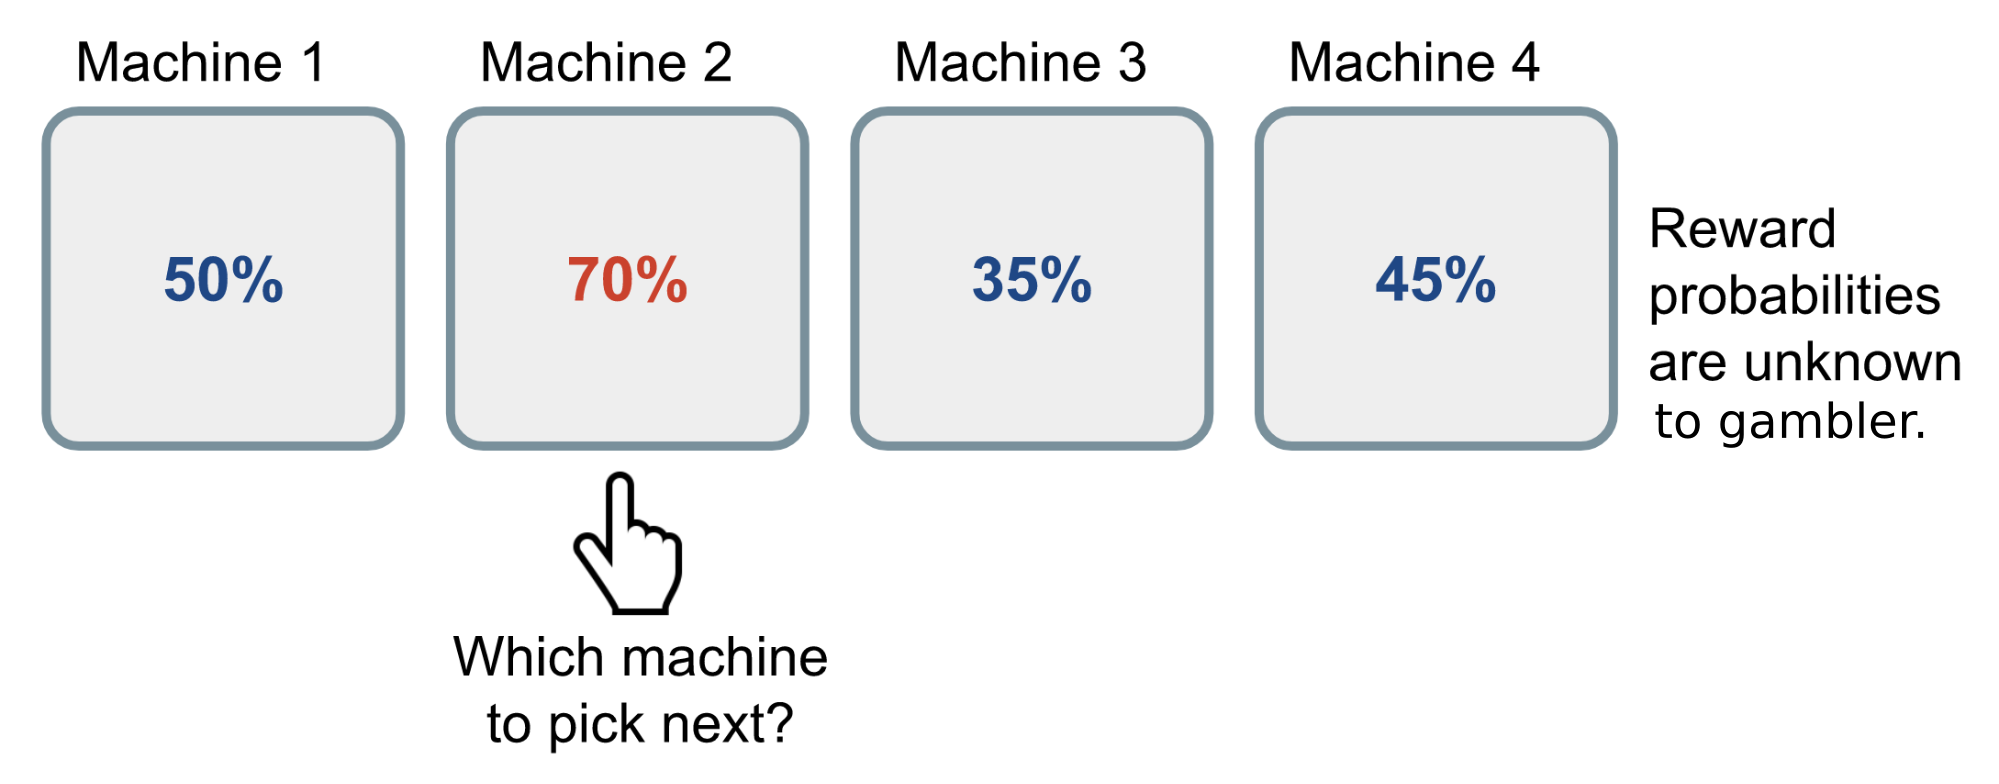
\includegraphics[width=4in]
{multi-armed/bern_bandit.png}
\caption{Bernoulli MAB (Bern-MAB)
with 4 arms. For a Bern-MAB, the 
conditional probability 
distribution $P(r|a)$ for reward $r$,
given  
arm $a$,
is initially totally unknown to the gambler (agent), 
but it is known by the environment to be
a Bernoulli distribution $P(r|a) = \mu_a^r(1-\mu_a)^{1-r}$
for $r\in \bool$, where $0<\mu_a<1$ for each $a$.
The percentages shown are $\mu_a$ for each arm $a$. }
\label{fig-bern-bandit}
\end{figure}

This chapter
is mostly based on Refs.
\cite{book-ashwin-rao} and \cite{weng2018bandit}.

Multi-armed Bandits (MABs) are a simple
version  of 
Reinforcement Learning (RL). RL is discussed 
in Chapter \ref{ch-RL}.

The term \qt{one-armed-bandit}
is a humorous term 
for what is also called
a slot machine.
A slot machine is a gambling device
which has a slot into which
you put coins or tokens
for the privilege of being allowed to  pull down 
a lever (arm) on one side of the device.
This action generates 
a random combination of three shapes, 
which may or may not, depending on their combination,
entitle the player to a 
 money award.

Multi-armed bandit (MAB)
is the name given to the 
optimization problem that considers an agent (gambler)
that
is playing multiple one-armed-bandits,
each with a possibly
different odds of winning.
The optimization problem is to determine
an efficient schedule
whereby the gambler can converge 
on the device with the highest odds of winning.




MABs are often used in marketing 
as an alternative to A/B testing.
These 2 methods yield different 
information but
overlap in that they 
both can discover consumer preferences.

The MAB problem is
an optimization problem (i.e., 
finding the maximum of 
a reward  function
or the minimum of a cost function).
As with any minimization problem,
an algorithm to solve it
runs the danger of
converging
to a local minimum
that isn't the global (i.e., 
the overall) minimum.
This danger can be diminished 
by doing both {\bf exploration
and exploitation}.
Algorithms that do no exploration,
only exploitation,
are said to be {\bf greedy},
and they are at the highest 
risk of converging to a non-global minimum.


\section{Bnet for MAB}
\begin{figure}[h!]
\centering
$$\xymatrix{
\rvs_{<0}\ar[r]\ar[d]&
\rvs_{<1}\ar[r]\ar[d]&
\rvs_{<2}\ar[d]&\cdots\\
\rva_0\ar[ur]\ar[d]&
\rva_1\ar[ur]\ar[d]&
\rva_2\ar[d]
\\
\rvr_0\ar[uur]&
\rvr_1\ar[uur]&
\rvr_2
}$$
\caption{Bnet for a multi-armed bandit (MAB).}
\label{fig-mab-bnet}
\end{figure}

Let 

$t\in \{0,1, 2, \ldots\}$ be the {\bf time}
 slice (step),

$\rva_t\in \{0, 1, \ldots, N_\rva-1\}=val(\rva)$
 be the {\bf arm} of bandit
that is pulled at time $t$, out of $N_\rva$ arms.
In RL language, it's also the {\bf action} taken.

$\rvr_t\in \RR$ be the {\bf reward} at time $t$,


$s_{<t} = [\underbrace{
(a_\tau, r_\tau)}_{s_\tau}: \tau<t]$
be the {\bf state} at time $t$.

Fig.\ref{fig-mab-bnet}
shows a bnet 
for a MAB.
The TPMs, printed in blue,
for this bnet, are as follows.


\beq\color{blue}
P(s_{<t}|s_{<t-1}, a_{t-1}, r_{t-1})) = 
\indi(s_{<t}= s_{<t-1}\cup (a_{t-1}, r_{t-1}))
\eeq
For $t=0$, $s_{<0}=\emptyset$, so
 choose a random $a_0$.

\beq\color{blue}
P(a_t|s_{<t})= \indi(a_t=a_t^*)
\;\;\text{(agent's response)}
\;,
\eeq
where $a^*_t$ depends on the
 {\bf strategy (a.k.a. policy)} being used
by the {\bf gambler (agent)}.
We consider various
strategies below.
$a^*_t$ is defined
solely in terms
of empirical data
(i.e., $a_t, r_t$
values)
collected from previous 
time-slices.
That is the only  type of
information that
the gambler 
is privy to.
$a_0^*$ is chosen at random.
The formulae for $a_t^*$
that we give below 
for various strategies
should only be used for $t>0$.

\beq\color{blue}
P(r_t|a_t) =
P_{\rvr|\rva}(r_t|a_t)
\;\;\text{(environment's response)}
\;.
\eeq
$P_{\rvr|\rva}$
is 
a probabilistic model that
models the {\bf environment}
in which the agent lives.
This 
assumes that the $a_t$ (and the $r_t$)
are i.i.d.
$P_{\rvr|\rva}$ 
depends on parameters
whose values are known
by the environment, 
but 
are not known
a priori
by the gambler.
In fact, the goal
of this exercise is for
the gambler to
 find 
ever more accurate 
estimates of those parameters,
using only the empirical 
data he/she can collect
from the past,
starting from total
ignorance about those parameters.


For a {\bf Bernoulli MAB (Bern-MAB)}, the 
conditional probability 
distribution $P_{\rvr|\rva}$
is
a Bernoulli distribution 

\beq
P(r|a) = \mu_a^r(1-\mu_a)^{1-r}
\eeq
for $r\in \bool$, where $0<\mu_a<1$ for each $a$.
The parameters $\mu_a$ are initially 
unknown to the gambler.
Note that $E[\rvr|a]=
\sum_r r P(r|a)=P(\rvr=1|a)=\mu_a$.

For a {\bf Gaussian MAB}, the 
conditional probability 
distribution $P_{\rvr|\rva}$
is
a Normal (Gaussian) distribution

\beq
P(r|a)=\caln(r; \mu_a, \s^2_a)
\;.
\eeq
for $r\in\RR$.
The parameters $\mu_a, \s^2_a$ are initially 
unknown to the gambler.
 
\section{Reward functions}




For $a\in val(\rva)$, define the
{\bf Long term Average Reward} for action $a$ by
\beq
\mu_a=Q(a)=E_{|a}[\rvr]=\sum_r r P(r|a)
\;.
\eeq
Let

\beq
a^* = \argmax_a Q(a)
\eeq

\beq
\mu^*=\max_a Q(a)=Q(a^*) 
\eeq

\beq
\Delta_a = \mu^*- Q(a)
\eeq
$\mu_a, a^*, \mu^*$ and $\Delta_a$
are not known to the gambler.


Define
the {\bf Instantaneous (at time $t$) Average
 Reward} for action $a$ by


\begin{subequations}
\label{eq-mab-q-n-eqs}
\beq
Q_{t}(a)=\frac{1}{N_{t}(a)}
\sum_{\tau=0}^{t} r_\tau
 \indi(a_\tau=a)
\label{eq-def-qt-a}
\eeq
where
\beq
N_{t}(a) =N_{in}+\sum_{\tau=0}^{t} 
\indi(a_\tau=a)
\eeq
\end{subequations}
$N_{in}>0$
insures that we never divide
by zero.
Note that Eqs.(\ref{eq-mab-q-n-eqs})
can be stated  recursively as

\begin{subequations}
\beq
N_t(a)Q_t(a)=
N_{t-1}(a)Q_{t-1}(a)+r_t \indi(a_t=a)
\eeq

\beq
N_t(a)=
N_{t-1}(a)+\indi(a_t=a)
\eeq
\end{subequations}
with $Q_{-1}(a)=0$
and $N_{-1}(a)=N_{in}$
for all $a$.
We assume that at large $t$, $N_{in}<<N_t(a)$
for all $a$.
For instance, one can use $N_{in}=1$.

$Q(a)$ 
is not known to the
gambler but
$N_{t}(a)$ and $Q_{t}(a)$ are
because they are empirical.

We will write a hat over 
random variables that are
defined by an empirical
probability distribution.\footnote{An
alternative convention
is to not
distinguish between $\HAT{\rva}_t$
and $\rva_t$,
or between $\HAT{\rvr}_t$
and $\rvr_t$,
but
to distinguish
between $P(r_t|a_t)$
and $\HAT{P}(r_t|a_t)$,
where $\HAT{P}()$
is an empirical estimate of $P()$.}
Whereas we assume that
$\rva_t$ and $\rvr_t$
are i.i.d., 
we will
not assume that $\hata_t$ and $\hatr_t$
are i.i.d.
for finite times $t$. What
we will  assume is that as $t\rarrow \infty$,

\beq
\HAT{\rva}_t\rarrow \rva
\;,\;
\HAT{\rvr}_t\rarrow \rvr
\eeq


Note that
\beq
\sum_a
\frac{N_t(a)}{t+1}=1
\eeq
so define

\beq
P(\HAT{\rva}_t=a)=\frac{N_t(a)}{t+1}
\;.
\eeq
Thus


\beq
E[Q(\HAT{\rva}_t)]=
\sum_a P(\HAT{\rva}_t=a)Q(a)
\;.
\eeq


\begin{claim}
\label{cl-qt-a-approx}
\beq
Q_t(a)= E_{|\HAT{a}_t=a}[\HAT{\rvr}_t]
\eeq
\end{claim}
\proof

Note that

\beq
\sum_{r}\sum_{\tau=0}^t
\frac{\indi(a_\tau=a, r_\tau=r)}{N_{t}(a)}
=1
\;.
\eeq
so define

\beq
P(\HAT{\rvr}_t=r|\HAT{\rva}_t=a)=
\sum_{\tau=0}^t
\frac{\indi(a_\tau=a, r_\tau=r)}{N_{t}(a)}
\;.
\eeq
Thus


\beqa
Q_{t}(a)&=&  \sum_r r
\sum_{\tau=0}^t
\frac{\indi(a_\tau=a, r_\tau=r)}{N_{t}(a)}
\\
&=&
\sum_r r
P(\HAT{\rvr}_t=r|\HAT{\rva}_t=a)
\\
&=&
E_{|\HAT{a}_t=a}[\HAT{\rvr}_t]
\eeqa
\qed


\begin{claim}
As $t\rarrow \infty$,

\beq
Q_t(a)\rarrow E_{\rva=a}[\rvr]=Q(a)
\eeq


\beq
E[Q(\HAT{\rva}_t)]\rarrow E[Q(\rva)]
\eeq

\end{claim}
\proof This is clear
from $\HAT{a}_t \rarrow a$
and $\HAT{r}_t \rarrow r$
and Claim \ref{cl-qt-a-approx}.
\qed


\section{Regret functions}

Define the
{\bf Instantaneous (at time $t$) Average Regret (I-Regret)} by
 
\beq
IReg_t =
\mu^* - E[Q(\HAT{\rva}_t)]
=
E[\Delta_{\HAT{\rva}_t}]
\eeq
and the {\bf Cumulative (for times $\leq t$) 
Average Regret  (C-Regret)} by
\beq
CReg_{t}=
\sum_{\tau=0}^t IReg_\tau
\;.
\eeq
Note that


\beqa
CReg_{t}&=&
\sum_{\tau=0}^t E[\Delta_{\HAT{\rva}_\tau}]
\\
&=&
\sum_a \Delta_a
\sum_{\tau=0}^t 
\frac{N_\tau(a)}{\tau+1}
\eeqa

Let

\beq
\rho_t=\frac{1}{t+1}
\sum_{t=0}^t r_t
\;.
\eeq
Define the {\bf Cumulative Average Reward (C-Reward)} by

\beq 
CRew_t= E_{|\HAT{\rva}_t=a}
[(t+1)\HAT{\ul{\rho}}_t]
\;.
\eeq
It can be shown that minimizing
the C-Regret
is equivalent to
maximizing
the C-Reward. 





\begin{claim}
As $t\rarrow \infty$,

\beq
IReg_t\rarrow E[\Delta_\rva]
\eeq

\end{claim}
\proof This is clear
from $\HAT{a}_t \rarrow a$
and $\HAT{r}_t \rarrow r$.
\qed

\section{Strategies with 
random exploration}
In this section,
we consider MAB algorithms
that explore
all values of the action $a$
at random.
In the section
following this one,
we consider MAB algorithm
that do a more deliberate
search of the action space.
\subsection{$\eps$-greedy algorithm}

Recall that $\rva_t\in \{0, 1, \ldots, N_\rva-1\}=val(\rva)$.
The user of the algorithm
 specifies
an $\eps\in [0,1]$
which measures the 
amount of exploration
to be conducted. 

\begin{figure}[h!]
$$
\xymatrix{
&\rvA_t\ar[dr]
\\
\rvg_t\ar[ru]\ar[rr]&&\rva_t
}
$$
\caption{Extra structure 
added to MAB Bnet Fig.\ref{fig-mab-bnet}
for $\eps$-greedy algorithm.}
\label{fig-mab-greedy-extra}
\end{figure} 


For each $t$, add extra the structure
shown in Fig.\ref{fig-mab-greedy-extra} to the MAB bnet 
Fig.\ref{fig-mab-bnet}.
$\rvg_t\in \bool$ and $\rva_t, \rvA_t\in val(\rva)$.
(\qt{g} stands for greedy).
The TPMs, printed in blue,
for the new nodes, are
as follows

\beq\color{blue}
P(g_t)=
\left\{
\begin{array}{ll}
\eps\;\;\text{(exploration)} & \text{if $g_t=0$}
\\
1-\eps\;\;
\text{(exploitation)}&\text{if $g_t=1$}
\end{array}
\right.
\;.
\eeq


\beq\color{blue}
P(A_t|g_t)=\left\{
\begin{array}{ll}
\frac{1}{N_\rva}\;\;\text{(exploration)}
&\;\;\text{if $g_t=0$}
\\
\indi(A_t=0)
\;\;\text{(exploitation)}&\;\;\text{if $g_t=1$}
\end{array}
\right.
\eeq

\beq\color{blue}
P(a_t|A_t, g_t)=\left\{
\begin{array}{ll}
\indi(a_t=A_t)\;\;\text{(exploration)}
&\;\;\text{if $g_t=0$}
\\
\indi(a_t=a^*_t)
\;\;\text{(exploitation)}&\;\;\text{if $g_t=1$}
\end{array}
\right.
\eeq
where $a^*_t$
is defined as follows:


\beq
\boxed{
a^*_t=
\argmax_a Q_{t-1}(a)}
\;.
\eeq

As $t\rarrow \infty$,
\beqa
\frac{N_t(a)}{t+1}
&=&P(\HAT{\rva}_t=a)
\\
&\rarrow&
P(a, g_t=0)\eps
+
P(a, g_t=1)(1-\eps)
\\
&\geq&
P(a, g_t=0)\eps
\\
&=&
\frac{\eps}{N_\rva}
\eeqa
Hence

\beqa
IReg_t &=& \sum_a \Delta_a\sum_{\tau=0}^{t} 
\frac{N_\tau(a)}{\tau+1}
\\
&\geq&
\frac{\eps}{N_\rva}
\sum_a\Delta_a
\eeqa
and
$CReg_t\geq\caln(!t)(t+1)$.
\subsection{$\eps_t$-greedy algorithm}
Replace time-independent constant
 $\eps$ in the 
$\eps$-greedy algorithm by
a time dependent 
function $\eps_t$.

\section{Strategies with
nonrandom exploration}

\subsection{Upper Confidence Bounds 
(UCB) algorithms}

A MAB algorithm
that maximizes merely 
$Q_t(a)$ to get
$a^*_t$ is totally greedy (i.e., does
no exploration,
only exploitation). 
This doesn't work too well
because once the 
algo finds 
a particular $a^*_t$,
it sticks with it.
For times $t$ after that,
the $Q_t(a)$ 
for all $a$ stay 
more or less the same.
The $N_t(a)$
for $a\neq a^*_t$
also
stay the same.
Only $N_t(a^*_t)$
increases.
To avoid this 
problem,
{\bf Upper Confidence Bounds 
(UCB) algorithms}
maximize  an effective
$Q_t(a)_{\rm eff}=
Q_t(a) + U_t(a)$,
where $U_t(a)>0$,
instead of maximizing
merely $Q_t(a)$
to get $a^*_t$.
$U_t(a)$ 
is proportional to
$1/\sqrt{N_t(a)}$
(that's a property of 
UCBs).
Adding $U_t(a)$
to $Q_t(a)$
gives those $a$
with low $N_a(a)$
a 
$Q_t(a)_{\rm eff}>> Q_t(a)$.
This encourages 
exploration
of $a$ 
different
from $a^*_t=\argmax Q_t(a)$.
In conclusion,
for  all UCB algorithms, we have

\beq
a^*_t=\argmax_a[Q_{t-1}(a) + U_{t-1}(a)]
\eeq
Different UCB algos
differ only in the
definition of $U_t(a)$.


Next, we consider
two UCB algorithms,
frequentist UCB (UCB1),
and Bayesian UCB.
 
\subsubsection{Frequentist UCB (UCB1)
algorithm}



\begin{claim}(Hoeffding’s Inequality- HI)
Let $\rvx_0, \rvx_1, \ldots, \rvx_{T-1}$
 be i.i.d. random variables 
such that $0\leq \rvx_t\leq 1$
for all $t$. 
Let $\rvm_{T-1}=\frac{1}{T}
\sum_{t=0}^{T-1} \rvx_t$ denote
the sample mean. Then for $u>0$,
we have:

\beq
P\left(E[\rvx]>\rvm_{T-1} + u\right)
\;\;\leq\;\; e^{-2Tu^2}
\;.
\eeq
\end{claim}
\proof
See Ref.\cite{wiki-hoeff}.
\qed

Let\footnote{As usual, we define
$\ZZ_{[a,b]}=\{a,a+ 1,a+2,  \ldots, b\}$
for $a<b$.
}

\beq
\rvx^T=\left\{\rvx_t:t\in\ZZ_{[0,T-1]} \right\}
\eeq
and

\beq
\rvr_{\leq t-1}(a)=
\{\rvr_\tau: \rva_\tau=a, 
\tau\in\ZZ_{[0, t-1]}\}
\;.
\eeq
Note that $\rvx^T$
has $T$ components and
 $\rvr_{\leq t-1}(a)$ has $N_{t-1}(a)$
components.
If we apply 
the HI with $\rvx^T$ replaced 
by $\rvr_{\leq t-1}(a)$, 
we get

\beq
P\left(Q(a)>Q_{t-1}(a) + U_{t-1}(a)
\right)\;\;\leq
\;\; e^{-2N_{t-1}(a)[U_{t-1}(a)]^2}
\eeq

If we define a threshold probability
 $p$
by

\beq
p= e^{-2N_{t-1}(a)[U_{t-1}(a)]^2}
\;,
\eeq
then

\beq
U_{t-1}(a)=\sqrt{
\frac{-\ln p}{2N_{t-1}(a)}}
\eeq

If we choose $p=(t-1)^{-\alp}$,


\beq
\boxed{
a_t^*=\argmax_a\left[Q_{t-1}(a) + \sqrt{
\frac{\alp (t-1)}{2N_{t-1}(a)}}
\;\;\right]
}
\eeq

\subsubsection{Bayesian UCB algorithm}

\begin{claim}\label{cl-b-updatng-normal}
\footnote{
For a {\bf standard deviation}
$\s$, the {\bf precision} $\tau$
is defined as $\tau=\frac{1}{\s^2}$.}
\footnote{
$\rvx|\lam\sim \cald(\lam)$
means that $P(x|\lam)=\cald(x;\lam)$.
$\caln()$ stands for the Normal distribution
and Gamma() for the Gamma distribution.
See Ref.\cite{wiki-gamma-dist}
for a discussion of the Gamma distribution.}
(Bayesian updating of mean and deviation.
See Fig.\ref{fig-bayes-updating-normal}.)

 
Suppose 

\beq 
x^n=[x_i]\;,\;\;x_i \text{ are i.i.d. with }
\ul{x_i}|\mu, \tau \sim \caln(\mu, \tau)
\eeq
\beq
\ul{\mu}|\tau \sim \caln(\mu_0, n_0\tau)
\eeq
\beq
\ul{\tau}\sim {\rm Gamma}(\alp, \beta)
\;.
\eeq
Then the posterior is

\beq
\ul{\mu}|\tau, x^n\sim
\caln\left(
\frac{n\ol{x}+n_0\mu_0}{n + n_0}\;\;,\;\;
(n+n_0)\tau
\right)
\eeq

\beq
\ul{\tau}|x^n\sim
{\rm Gamma}
\left(
\alp +\frac{n}{2}\;\;,\;\;
\beta +\frac{1}{2}
\sum_i(x_i - \ol{x})^2
+
\frac{nn_0}{2(n+n_0)}(\ol{x}-\mu_0)^2
\right)
\eeq
\end{claim}
\proof See Ref.\cite{jordan-b-updating}.
\qed
 
\begin{figure}[h!]
\centering
$$\xymatrix{
\ul{\alp}\ar[dr]
&&\ul{\beta}\ar[dl]
&&\ul{\mu}_0\ar[dr]
&&\ul{\tau}_0\ar[dl]
\\
&\stackrel{\rm Gamma}{\ul{\tau}}
\ar[drr]\ar[rrrr]
&&&&\stackrel{\rm Normal}{\ul{\mu}}\ar[dll]
\\
&&&\stackrel{\rm Normal}{\rvx^n}
}
\;\;\;
\xymatrix{
\\
\stackrel{\rm Gamma}{\ul{\tau}}
\ar[rr]&&
\stackrel{\rm Normal}{\ul{\mu}}
\\
&\rvx^n\ar[ur]\ar[ul]
}$$
\caption{
Prior and Posterior
Bnets in Claim
 \ref{cl-b-updatng-normal}.}
\label{fig-bayes-updating-normal}
\end{figure}

In the Bayesian UCB algorithm, we use

\beq
\boxed{a^*_t=
\argmax_a E_{\mu_a, \s_a|s_{< t}}\left[\mu_a
+
c\frac{\s_a}{\sqrt{N_{t-1}(a)}}\right]}
\label{eq-gauss-mab-a-star}
\eeq
for some $c>0$.

Eq.\ref{eq-gauss-mab-a-star}
requires that we know
 $P(\mu_a, \s_a|s_{< t})$
; i.e., the posterior distribution
of $\mu_a, \s_a$ assuming
the prior history $s_{< t}$.
This follows from Bayes theorem
if we assume a Normal distribution
for the likelihood $P(s_{< t}|\mu_a, \s_a)$
and we assume
conjugate priors for $P(\mu_a, \s_a)$.
More precisely,
if we replace $\rvx^n$
by $\rvs_{< t}$
in Claim \ref{cl-b-updatng-normal},
then
\beq
P(\mu_a, \tau_a|s_{< t})=
P(\mu_a|\tau_a, s_{< t})P(\tau_a|s_{< t})
\eeq
where
$P(\mu_a|\tau_a, s_{< t})$
and $P(\tau_a|s_{< t})$
are given by 
Claim \ref{cl-b-updatng-normal}.



\subsection{Thompson Sampling MAB
 (TS-MAB)
algorithm}

\subsubsection{Bnet for general TS-MAB
algorithm}
\begin{figure}[h!]
$$\xymatrix{
\rvs_{<0}\ar[r]\ar[d]
&
\rvs_{<1}\ar[r]\ar[d]
&
\rvs_{<2}\ar[d]&\cdots
\\
\ul{\lam}_0\ar[d]\ar[r]
&\ul{\lam}_1\ar[d]\ar[r]
&\ul{\lam}_2\ar[d]
\\
\rva_0\ar[uur]\ar[d]&
\rva_1\ar[uur]\ar[d]&
\rva_2\ar[d]
\\
\rvr_0\ar[uuur]&
\rvr_1\ar[uuur]&
\rvr_2
}$$
\caption{Bnet for TS-MAB
 algorithm.}
\label{fig-bnet-thom-mab}
\end{figure}
The Thompson Sampling MAB (TS-MAB)
algorithm is described by
the bnet 
Fig.\ref{fig-bnet-thom-mab}.
This bnet differs from the bnet
Fig.\ref{fig-mab-bnet}
in that it
includes new nodes $\ul{\lam}_t$.
The TPMs, printed in blue,
for bnet
Fig.\ref{fig-bnet-thom-mab}, 
are as follows.

\beq\color{blue}
P(s_{<t}|s_{<t-1},a_{t-1}, r_{t-1})=
\text{ same as for Fig.\ref{fig-mab-bnet}}
\eeq

\beq\color{blue}
P(\lam_t|s_{<t}, \lam_{t-1})=
\indi(\lam_t=\lam^*_t(s_{<t},\lam_{t-1}))
\eeq
where $\lam^*_t$ is a function
to be defined below.

\beq\color{blue}
P(a_t|\lam_t)=\indi[a_t=a_t(\lam_t)]
\;\;\text{(Agent's response)}
\eeq
where $a_t(\lam_t)$
is a function
to be described below.

\beq\color{blue}
P(r_t|a_t)=
\text{ same as for Fig.\ref{fig-mab-bnet}.
(Environment's response)}
\eeq

Let

\beqa
Q_{t}(a,\lam_t)&=&
\sum_r r P(\HAT{\rvr}_{t}=r|\HAT{\rva}_t=a, \lam_t)
\\
&=&
E_{|\HAT{\rva}_t=a, \lam_t}[\HAT{\rvr}_{t}]
\;.
\eeqa
Define

\beq
\boxed{
a_t(\lam_t)
=
\argmax_a Q_{t}(a,\lam_t)}
\;.
\eeq
Note that

\begin{subequations}
\label{eq-ts-wo-lam-delta}
\beqa
P(a_t|s_{<t})
&=&
\sum_{\lam_t}P(\lam_t|s_{<t})
\indi[Q_t(a_t, \lam_t)=
\max_a Q_t(a, \lam_t)]
\\
&=&
\sum_{\lam_t}P(\lam_t|s_{<t})
\indi[a_t=a_t(\lam_t)]
\\
&=&
E_{\lam_t|s_{<t}}\{
\indi[a_t=a_t(\lam_t)]
\}
\;.
\eeqa
\end{subequations}
If we further assume that 
$P(\lam_t|s_{<t})$ is a delta function,
then Eqs.(\ref{eq-ts-wo-lam-delta}) reduce  to


\beq
P(a_t|s_{<t})
=
\indi[a_t=a_t(\lam^*_t)]
\label{eq-ts-with-lam-delta}
\eeq


\subsubsection{TS-MAB algorithm with
Beta agent and Bernoulli environment}
The Beta distribution ${\rm Beta}(x;\alp, \beta)$ 
(see Ref.\cite{wiki-beta-dist}) is defined
for $\alp>0, \beta>0$ and $x\in[0,1]$.
Since $x\in [0,1]$,
$x$ can be interpreted as a probability.
The mean and variance of the Beta distribution
are

\beq
E[\rvx]=\frac{\alp}{\alp+\beta}
\;,
\eeq

\beq
\av{\rvx, \rvx}=
\frac{\alp\beta}
{(\alp+\beta)^2(\alp+\beta+1)}
\;.
\eeq
From this mean and variance, 
we see that if we increase $\alp$
by one and leave $\beta$ the same, 
the mean moves towards 1
and the variance decreases.
Likewise, if we increase $\beta$ by
1 and leave $\alp$ the same, 
the mean moves towards 0 and 
the variance decreases.

Let

\beq
\alp^a_t=\sum_{\tau=0}^{t}\indi(r_\tau=1, a_\tau=a)
\eeq

\beq
\beta^a_t=\sum_{\tau=0}^{t}\indi(r_\tau=0, a_\tau=a)
\eeq

\beq
\lam^a_t=(\alp^a_{t-1}, \beta^a_{t-1})
\eeq

\beq
\lam_t=[(\alp^a_{t-1}, \beta^a_{t-1}): a\in val(\rva)]
\eeq

\begin{subequations}
\label{eq-qt-beta-bern}
\beqa
Q_t(a, \lam_t)
&=&\sum_r r 
{\rm Beta}(r;\alp^a_{t-1}, \beta^a_{t-1})
\\
&=&
\frac{\alp^a_{t-1}}{
\alp^a_{t-1} + \beta^a_{t-1}
}
\eeqa
\end{subequations}

The TS-MAB 
algorithm 
for a Beta agent and
Bernoulli
environment
can be described
by the bnet 
Fig.\ref{fig-bnet-thom-mab}.
For this special case
of bnet Fig.\ref{fig-bnet-thom-mab},
the TPMs, printed in blue,
are as follows.

\beq\color{blue}
P(s_{<t}|s_{<t-1},a_{t-1}, r_{t-1})=
\text{ same as for
 Fig.\ref{fig-bnet-thom-mab}}
\eeq


\beq\color{blue}
P(\lam^a_t|s_{<t}, \lam_{t-1})=
\indi(\lam^a_t=\lam^{*a}_t)=
\left\{
\begin{array}{ll}
\indi(\lam^a_{t}=\lam^a_{t-1})
&\text{if $a\neq a_{t-1}$}
\\
\indi(\lam^a_{t}=(\alp^a_{t-2} +1, \beta^a_{t-2}))
&\text{if $a_{t-1}=a$ and $r_{t-1}=1$}
\\
\indi(\lam^a_{t}=(\alp^a_{t-2}, \beta^a_{t-2}+1))
&\text{if $a_{t-1}=a$ and $r_{t-1}=0$}
\end{array}
\right.
\eeq


\begin{align}\color{blue}
P(\rva_t|\lam_t)
&\color{blue}= \indi( a_t=a_t(\lam_t))
\\
&\color{blue}= \indi( a_t=\argmax_a
\underbrace{ Q_t(a, \lam_t)}_
{\text{see Eq.(\ref{eq-qt-beta-bern}).}}
)
\;\;\text{(Beta agent response)}
\end{align}

\beq\color{blue}
P(r_t|a_t) =
\mu_{a_t}^{r_t}(1-\mu_{a_t})^{r_t}
\;\;\text{(Bernoulli environment response)}
\;.
\eeq
$\mu_a$ known to environment
but unknown to agent.

\subsubsection{TS-MAB 
algorithm, skeletal reprise}

The TS-MAB algorithm
is not very 
complicated but explaining
it with precision
requires nightmarishly many
indices.
Here is a pedagogical reprise
of what we have said so far,
where we have 
stripped out some of the
inessential indices.




\beq
P(\lam)=\indi(\lam, \lam^*)
\eeq

\beqa
P(a|\lam)
&=&\indi(a=a(\lam))
\\
&=&\indi(a=\argmax_a \sum_r r P(\HAT{r}=r|\HAT{a}=a, \lam))
\\
&=& \indi( a=\argmax_a \sum_r r {\rm Beta}(r; \lam^a))
\;\;\text{(Beta agent response)}
\eeqa

Define $q()$ by
\beq
q(r;\lam^a)=P(\HAT{r}=r|\HAT{a}=a, \lam)
\eeq

\begin{itemize}
\item PRIOR:
\beqa
P(a)&=&
\sum_\lam P(\lam)P(a|\lam)
\\
&=&
P(a|\lam^*)
\\
&=&
\indi( a=\argmax_a
 \sum_r r q(r; \lam^{*a})
\eeqa


\begin{enumerate}
\item Use fact that $q=$Beta
\beq
\sum_r r {\rm Beta}(r; \lam^{*a})
=
\frac{\alp^{*a}}{\alp^{*a}+\beta^{*a}}
\eeq

\item Don't use fact that $q=$Beta.

 For each $a$,
get samples $r^\s \sim
q(r; \lam^{*a})$
for $\s=0, 1, \ldots, nsam-1$
and estimate

\beq
\sum_r r q(r; \lam^{*a})
\approx
\frac{1}{nsam}\sum_\s
r^\s q(r^\s; \lam^{*a})
\;.
\eeq
This sampling is why TS is called a sampling.
\end{enumerate}


\item LIKELIHOOD:
\beq
P(r|a) =
\mu_{a}^{r}(1-\mu_{a})^{r}
\;\;\text{(Bernoulli environment response)}
\eeq
\end{itemize}



\subsection{Grad-MAB algorithm}

Let

\beq
\lam_{t+1}(a)
=
\lam_{t}(a)
+ \eta
r_{t}[\indi(a_{t}=a)-
\pi_{t}(a)]
\label{eq-mab-lam-recur}
\eeq
for some $\eta>0$, where
$\pi_t(a)$ is defined by

\beq
\pi_t(a)=
P(\rva_t=a|\lam_t)=
\underbrace{\frac{e^{\lam_t(a)}}{\sum_a
e^{\lam_t(a)}}
}_{
\softmax(\lam_t)(a)}
\;.
\eeq
The $\lam_t(a)$ are called {\bf scores}
at time $t$. 
Let

\beq
\boxed{
a^*_t = \argmax_a \pi_t(a)}
\eeq

\begin{figure}[h!]
$$\xymatrix{
\rvs_{<0},\ul{\lam}_0\ar[r]\ar[d]&
\rvs_{<1},\ul{\lam}_1\ar[r]\ar[d]&
\rvs_{<2},\ul{\lam}_2\ar[d]&\cdots\\
\rva_0\ar[ur]\ar[d]&
\rva_1\ar[ur]\ar[d]&
\rva_2\ar[d]
\\
\rvr_0\ar[uur]&
\rvr_1\ar[uur]&
\rvr_2
}$$
\caption{Bnet for Grad-MAB algorithm. }
\label{fig-bnet-grad-mab}
\end{figure}

The Gradient MAB (Grad-MAB)
algorithm is described by
the bnet 
Fig.\ref{fig-bnet-grad-mab}.
This bnet differs from the bnet
Fig.\ref{fig-mab-bnet}
in that it
includes new nodes $\ul{\lam}_t$.
The TPMs, printed in blue,
for bnet
Fig.\ref{fig-bnet-grad-mab}, 
are as follows.

\beq\color{blue}
P(\ul{\lam}_{t+1}=\lam|a_t, r_t, \lam_t)=
\indi(\lam= \lam_{t+1} \text{ given by 
Eq.(\ref{eq-mab-lam-recur}).}
\eeq


\beq\color{blue}
P(a_t|\lam_t)
=\indi(a_t=a^*_t)
\text{\;\;\;or, alternatively,}
=P(\rva_t=a_t|\lam_t)=\pi_t(a_t)
\;\;\text{(agent's response)}
\eeq

\beq\color{blue}
P(r_t|a_t) =
P_{\rvr|\rva}(r_t|a_t)
\;\;\text{(environment's response)}
\;.
\eeq


Motivation:





Define the {\bf Instantaneous
Average Reward} by

\beq
\calr_t(\lam_t)=
\sum_a P(\rva_t=a|\lam_t) E_{\rvr_t|\rva_t=a}[\rvr_t]
=E_{\rvr_t,\rva_t|\lam_t}[\rvr_t]
\;.
\eeq

We will assume that as $t\rarrow \infty$,
$\rva_t\rarrow \rva$,  
$\rvr_t\rarrow\rvr$
and $\lam_t\rarrow \lam$.
Therefore, $\calr_t(\lam_t)\rarrow
E_{\rvr,\rva|\lam}[\rvr]
=E_{\rvr|\lam}[\rvr]$.

Note that if
$E_{\rvr_t|\rva_t=a}[\rvr_t]=B$,
where $B$ is independent of $a$,
then $\calr_t(\lam_t)=B$
and $\pder{\calr_t}{\lam_t(a)}=0$.



\begin{claim}
\label{cl-grad-r-grad-mab}
The gradient of $\calr_t(\lam_t)$ is

\beq
\pder{\calr_t}{\lam_t(a)}
=
E_{\rvr_t,\rva_t|\lam_t}
[g(\rvr_t,\rva_t|a,\lam_t)]
\eeq
where
\beq
g(\rvr_t,\rva_t|a,\lam_t)=\rvr_t[
\indi(\rva_t=a) -\pi_t(a)]
\eeq

\end{claim}
\proof

\beqa
\pder{\calr_t}{\lam_t(a)}
&=&
\sum_{a'} \pder{\pi_t(a')}{\lam_t(a)}
E_{\rvr_t|\rva_t=a'}[\rvr_t]
\\
&=&
\sum_{a'}\pi_t(a') \pder{\ln \pi_t(a')}{\lam_t(a)}
E_{\rvr_t|\rva_t=a'}[\rvr_t]
\\
&=&
\sum_{a'}\pi_t(a') \pder{}{\lam_t(a)}\left[\ln
\frac{\exp[\lam_t(a')]}{\sum_a
 \exp[\lam_t(a)]}\right]
E_{\rvr_t|\rva_t=a'}[\rvr_t]
\\
&=&
\sum_{a'}\pi_t(a') [\indi(a'=a)-\pi_t(a)]
E_{\rvr_t|\rva_t=a'}[\rvr_t]
\\
&=&
\sum_{a'}P(\rva_t=a'|\lam_t)
E_{\rvr_t|\rva_t=a'}[\rvr_t(\indi(a'=a)-\pi_t(a))]
\\
&=&
E_{\rvr_t,\rva_t|\lam_t}
[g(\rvr_t,\rva_t|a,\lam_t)]
\eeqa
\qed

Eq.(\ref{eq-mab-lam-recur}) 
can be written as
\beq
\lam_{t+1}(a)
=
\lam_{t}(a)
+ \eta
g(r_t,a_t|a,\lam_t)
\eeq
